%\todofilebegin{040\_evaluation\_validation.tex}
%%%%%%%%%%%%%%%%%%%%%%%%%%%%%%%%%%%%%%%%%%%%%%%%%%%%%%%%%%%%%%%%%%%%%%%%%%%%%%
%%%%%%%%%%%%%%%%%%%%%%%%%%%%%%%%%%%%%%%%%%%%%%%%%%%%%%%%%%%%%%%%%%%%%%%%%%%%%%
%%%%%%%%%%%%%%%%%%%%%%%%%%%%%%%%%%%%%%%%%%%%%%%%%%%%%%%%%%%%%%%%%%%%%%%%%%%%%%

\section{Evaluation and Validation}

SOSflow is a large, complex, and completely new tool framework. The
core library components comprise more than 12,000 lines of original
C99 code. SOSflow's code base has \textit{not} been systematically
optimized for this pre-release research work -- since it is an open
source project, volunteers are always welcome! It is likely that the
observed performance of SOSflow will dramatically improve with several
iterations of focused overhead and latency refactoring. Many of the
behavioral characteristics of SOSflow are the product of its internal
parameters and the configuration of its runtime deployment, rather
than products of its data model and algorithms. The exploration of
optimal settings in that combined parameter space is left for future
work: For now the effort was made to select reasonable default SOSflow
configuration parameters and typical/non-priviledged cluster
queues and topologies.

SOSflow as a tool is \textit{production capable} for the purpose of
validating the SOS workflow performance model. As we demonstrate, even
the current un-optimized code is able to scale out to reasonable
allocation sizes and handle relatively impressive varieties,
quantities, and rates of data flow. Because of the lack of focused
tuning to its internal mechanics and the general novelty of the
architecture, the results and figures presented here should be
considered the \textit{worst-case scenario} for the performance of
SOSflow itself, now and for the future.

%-----------------------------------------------------------------------------
\subsection{Testing Platform and SOS Configurations}

Single node tests of SOSflow were performed by launching the
sosd(listener) daemon along with an sosd(db) instance as background MPI tasks.
The demo\_app tool was then also launched as an MPI task with varying parameters
to explore the capabilities of the sosd daemons.

\todo[inline]{...}

%-----------------------------------------------------------------------------
\subsection{Latency}

\todo[inline]{...}

\begin{figure}[!t]
\centering
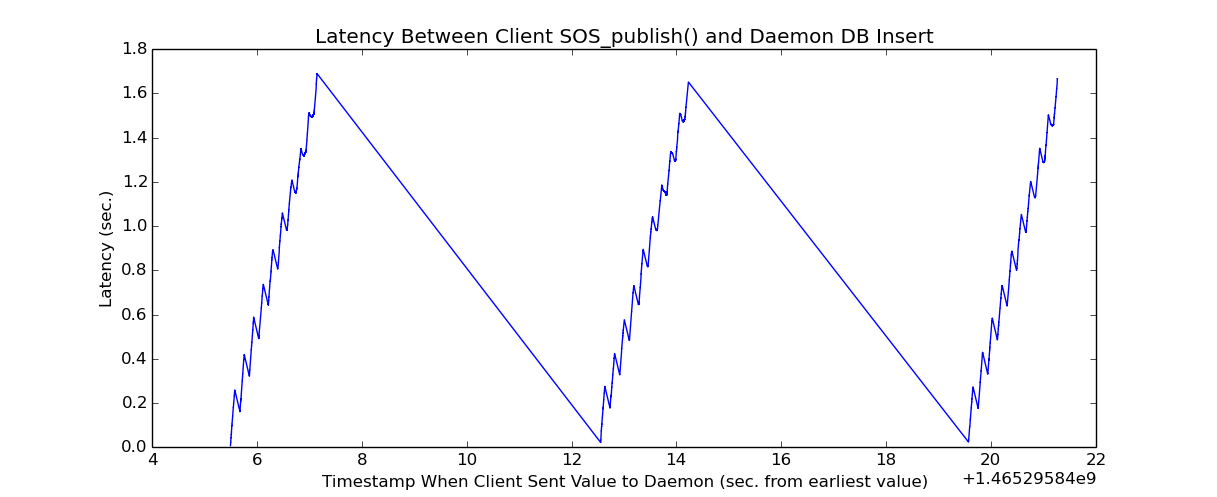
\includegraphics[width=2.5in]{images/aciss_latency_3_situ.png}
\caption{In Situ Latency (3 Nodes, 30 Applications)}
\label{fig_sim}
\end{figure}

\begin{figure}[!t]
\centering
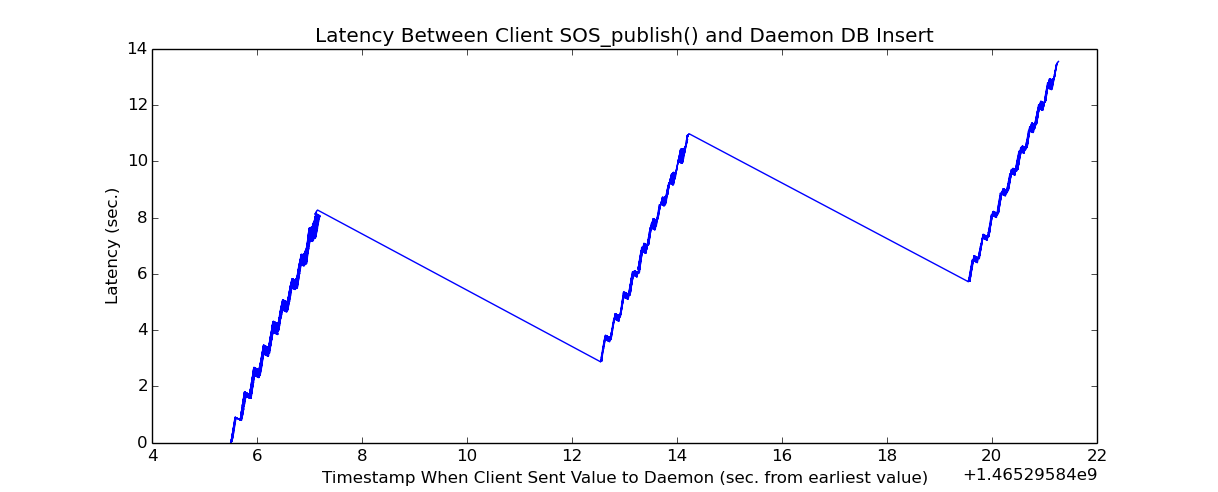
\includegraphics[width=2.5in]{images/aciss_latency_3_agg.png}
\caption{Aggregate sosd(db) Latency (3 Nodes, 30 Applications)}
\label{fig_sim}
\end{figure}

\begin{figure}[!t]
\centering
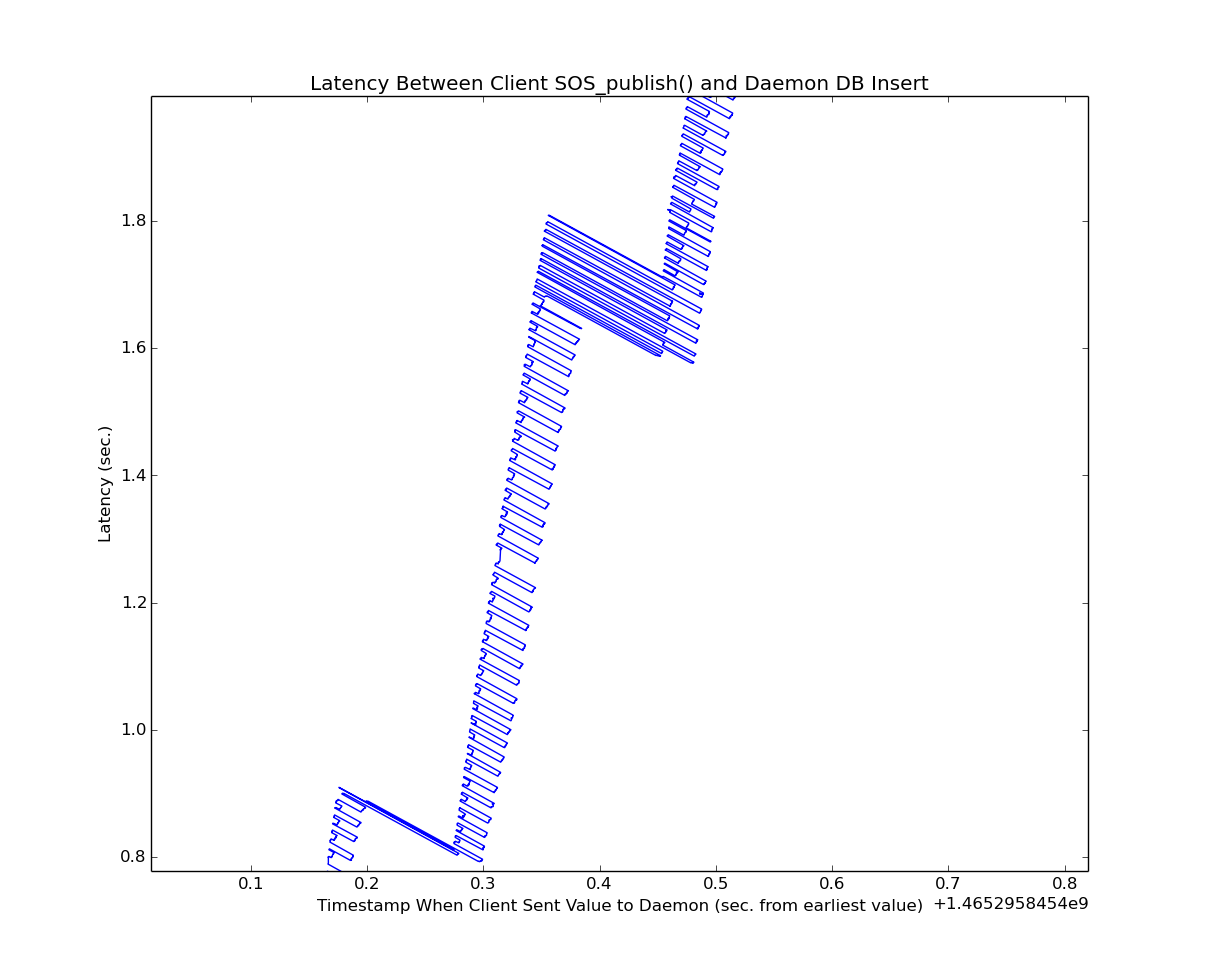
\includegraphics[width=2.5in]{images/aciss_latency_3_agg_zm.png}
\caption{Aggregate sosd(db) Detail (3 Nodes, 30 Applications)}
\label{fig_sim}
\end{figure}


\begin{figure}[!t]
\centering
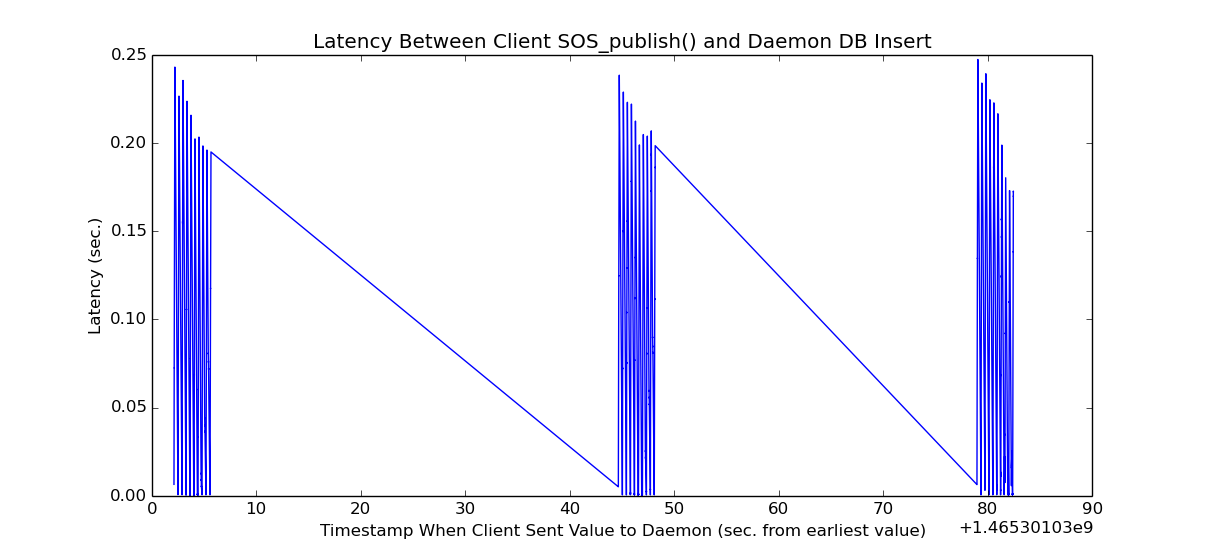
\includegraphics[width=2.5in]{images/aciss_latency_24_situ.png}
\caption{In Situ Latency (24 Nodes, 240 Applications)}
\label{fig_sim}
\end{figure}


\begin{figure}[!t]
\centering
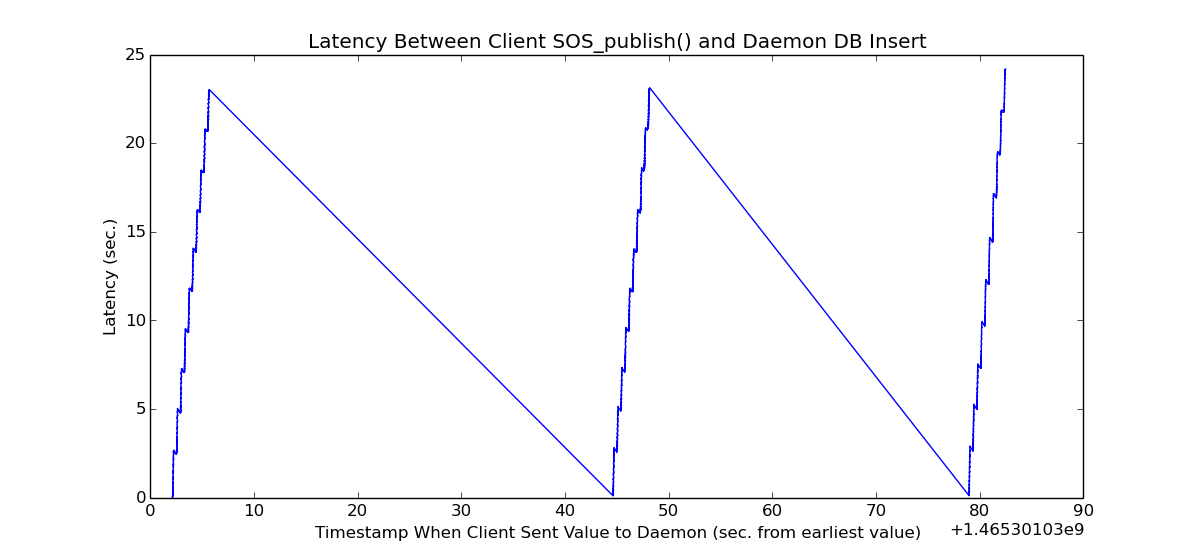
\includegraphics[width=2.5in]{images/aciss_latency_24_agg.png}
\caption{Aggregate sosd(db) Latency (24 Nodes, 240 Applications)}
\label{fig_sim}
\end{figure}



%-----------------------------------------------------------------------------
\subsection{Scalability}

\todo[inline]{...}

\begin{figure}[!t]
\centering
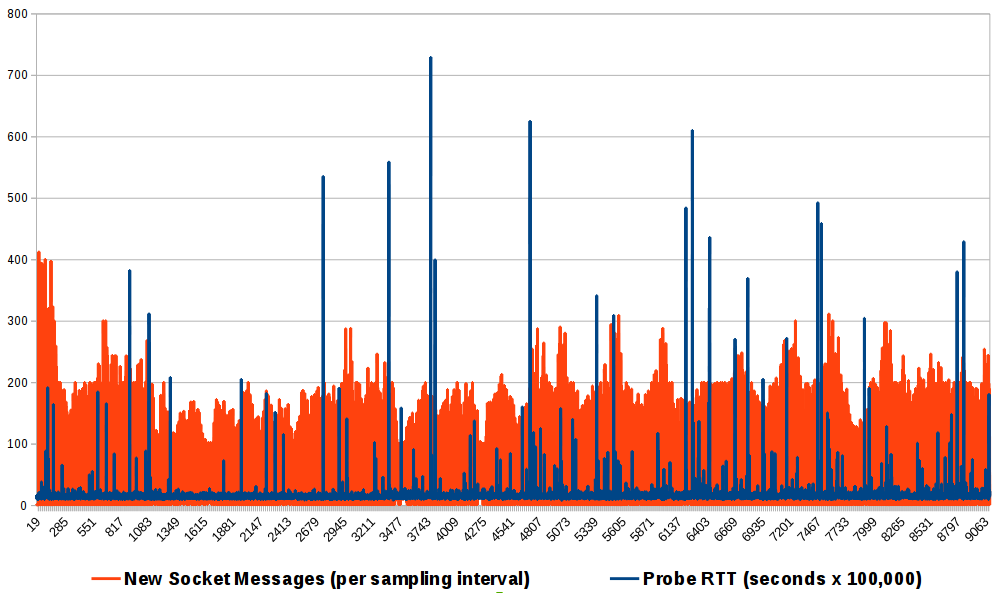
\includegraphics[width=2.5in]{images/icebox_api_cost_when_slam.png}
\caption{SOSflow Socket Communication Cost (~0.003sec)}
\label{fig_sim}
\end{figure}


\begin{figure}[!t]
\centering
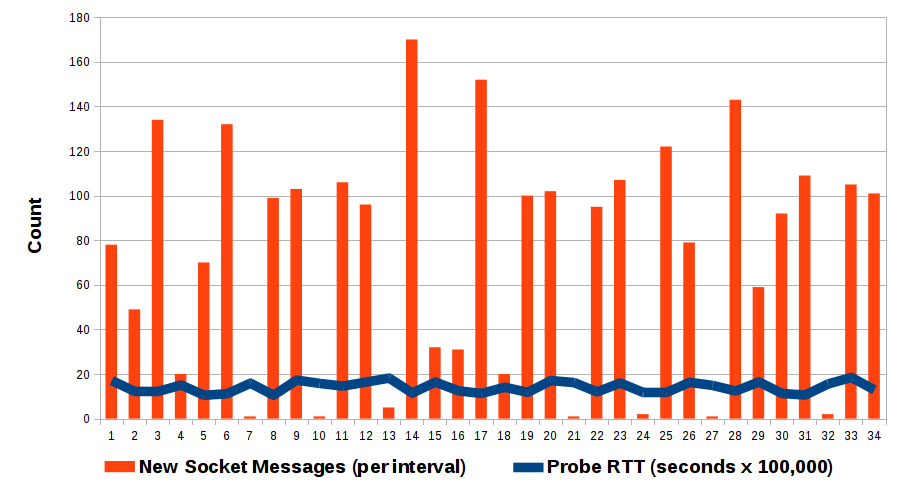
\includegraphics[width=2.5in]{images/icebox_api_cost_zoom.png}
\caption{SOSflow Socket Communication Cost, Detail}
\label{fig_sim}
\end{figure}




%-----------------------------------------------------------------------------
\subsection{Overhead and Perturbation}

\todo[inline]{...}

%\todofileend{040\_evaluation\_validation.tex}
